\cleardoublepage

\chapter {Wireshark}

% DON'T FORGET TO TRANSLATE THE FOOTNOTE
\lgf{\Index{Wireshark} va être notre ami dans la suite de cet ouvrage pour comprendre le fonctionnement des protocoles et analyser les données qui vont circuler. Malheureusement, dans certains cas, nous devons avoir recours à des outil plus rustiques comme des traces en \Index{hexadécimal}\footnote{\url{https://fr.wikipedia.org/wiki/Syst\%C3\%A8me\_hexad\%C3\%A9cimal}} (base 16).  Il faut donc se familiariser avec ces outils, ce que nous allons faire dare-dare en analysant des requêtes HTTP simples. Si vous avez accès à un ordinateur pouvant faire tourner Wireshark, nous vous recommandons d'essayer de faire les manipulation indiquées et de répondre aux questions.}
\lge{\Index{Wireshark} is going to be our friend in the rest of this book. It will help us to understand the protocols and to analyze the data which will circulate. Unfortunately, in certain cases, we must resort to more rustic tools such as traces in \Index{hexadecimal}\footnote{\url{https://en.wikipedia.org/wiki/Hexadecimal}} (base 16).  It is thus necessary to become familiar with these tools. We will do straight away by analyzing simple HTTP requests. If you have access to a computer that can run Wireshark, we recommend that you try to do the manipulations described bellow and answer the questions.}


\section{Installation}

\lgf{L'installation de Wireshark se fait en allant sur le site éponyme \url{https://www.wireshark.org/}, soit sous Linux en installant le paquetage \texttt{wireshark}. Ce programme nécessite des droits particuliers pour accéder aux messages venant du réseau, il faut les accorder au moment de l'installation.}
\lge{The installation of Wireshark is done by going on the eponymous site \url{https://www.wireshark.org/}, or under Linux by installing the package \texttt{wireshark}. This program requires particular rights to access messages coming from the network, you must grant them at the time of the installation.}


\lgf{\section{Démarrage}}
\lge{\section{Startup}}


\lgf{Si vous lancez Wireshark avec les bon privilèges, la fenêtre d'accueil va afficher les interfaces disponibles, comme le montre la figure~\vref{fig-wires-open} sur Windows. En regard avec le modèle de référence de l'\ac{ISO}, il s'agit des protocoles de niveau 2 présent sur l'ordinateur. Il peut s'agit d'une carte physique comme Ethernet ou Wi-Fi ou d'interface virtuelle utilisées pour communiquer en interne sur l'ordinateur. }
\lge{If you launch Wireshark with the right privileges, the welcome window will display the available interfaces, as shown in the figure~\vref{fig-wires-open} on Windows. Compared to the reference model of the ISO, these are all the level 2 interfaces present on the computer. It can be a physical card like Ethernet or Wi-Fi or a virtual interface used to communicate internally on the computer. }


\begin{figure}[tbp]
\centerline{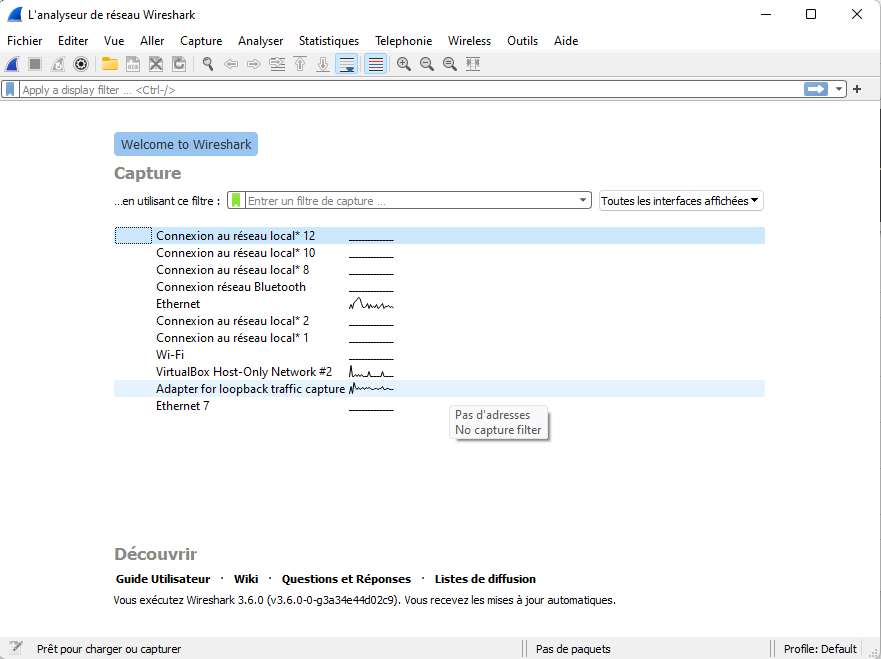
\includegraphics[width=1\columnwidth]{Pictures/wireshark-open.png}}
\lgf{\caption{Ouverture de Wireshark}}
\lge{\caption{Wireshark opening}}
\label{fig-wires-open}
\end{figure}


\lgf{Il s'agit de déterminer quelle interface choisir. Ce n'est pas toujours facile car leurs noms ne sont pas toujours très explicites. Les petites courbes à gauche du nom indiquent le trafic instantané que Wireshark mesure. Sur le schéma, 3 interfaces sont actives : Ethernet, la communication avec une machine virtuelle et une interface appelée \textit{\Index{loopback}}.  La première permet d'avoir les communications avec l'extérieur et la dernière sera très utile lors des échanges entre deux processus dans cette machine.}
\lge{It is a question of determining which interface to choose. This is not always easy because their names are not always very explicit. The small curves on the left of the name indicate the instantaneous traffic that Wireshark measures. On the diagram, 3 interfaces are active: Ethernet, communication with a virtual machine and an interface called \textit{Index{loopback}}.  The first one allows to have the communication with the outside and the last one will be very useful during the exchanges between two processes in this machine.}


\section {Capture}

\lgf{En cliquant sur le nom de l'interface donnant accès au réseau exterieur (\Index{Ethernet} dans notre cas), la fenêtre se découpe en 3 parties, comme le montre la figure~\vref{fig-wires-cap}.}
\lge{By clicking on the name of the interface giving access to the external network (\Index{Ethernet} in our case), the window splits into 3 parts, as shown in the figure~\vref{fig-wires-cap}.}


\begin{figure}[tbp]
\centerline{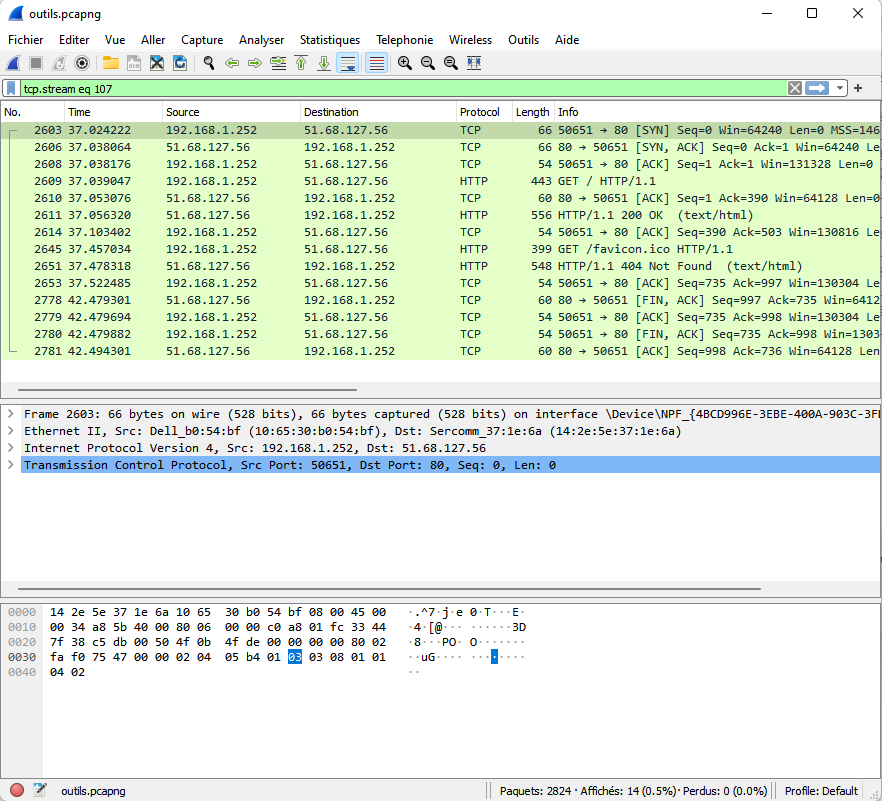
\includegraphics[width=1\columnwidth]{Pictures/ws-capture.png}}
\lgf{\caption{Capture du trafic}}
\lge{\caption{Traffic Capture}}
\label{fig-wires-cap}
\end{figure}

\lgf{L'écran de Wireshark se divise en 3 parties~:}
\lge{The Wireshark screen is divided into 3 parts:}
\begin{itemize}
\item 
    \lgf{en haut, défile les trames qui sont capturées sur le réseau, chaque protocole à une couleur dédiée pour facilité le repérage~:}
    \lge{at the top, scrolls the frames that are captured on the network, each protocol has a dedicated color for easy identification:}
    
    \begin{itemize}
    \item 
        \lgf{le numéro de trame capturée, il s'agit d'une information ajoutée par Wireshark,}
        \lge{the captured frame number, this is an information added by Wireshark,}
    \item 
        \lgf{l'heure de capture de la trame. Cette information est aussi ajoutée par Wireshark,}
        \lge{the time of capture of the frame. This information is also added by Wireshark,}
    \item 
        \lgf{l'adresse IP (IPv4 ou IPv6) de la machine à l'origine du paquet,}
        \lge{the IP address (IPv4 or IPv6) of the machine originating the packet,}
    \item 
        \lgf{l'adresse IP (IPv4 ou IPv6) de la machine destinataire du paquet,}
        \lge{the IP address (IPv4 or IPv6) of the machine receiving the packet,}
    \item 
        \lgf{le protocole de plus haut niveau contenu dans la trame. Dans notre cas, cela peut être TCP si le message TCP ne contient pas de données, comme lors de l'ouverture de connexion, ou de certains acquittements. On voit également les messages \ac{HTTP} qui sont bien entendu encapsulés dans TCP,}
        \lge{the highest level protocol contained in the frame. In our case, this can be TCP if the TCP message does not contain data, as in the case of connection opening, or certain acknowledgements. We also see the messages \ac{HTTP} which are of course encapsulated in TCP,}
    \item 
        \lgf{la taille en octets de la trame capturée par Wireshark,}
        \lge{the size in bytes of the frame captured by Wireshark,}
    \item 
        \lgf{finalement Wireshark fourni un résumé du contenu de la trame, pour comprendre ce qui se passe sur le réseau. Dans la capture, on retrouve pour les messages \ac{HTTP}, les requêtes GET ou les notifications~;}
        \lge{Finally Wireshark provides a summary of the content of the frame, to understand what is happening on the network. In the screenshot, we can see for the messages, the GET requests or the notifications;}
    \end{itemize}

\item 
    \lgf{si une trame est sélectionnée dans la liste, elle apparaît dans la zone du milieu avec l'empilement protocolaire. Le contenu de chacun de ces protocoles peut être détaillé en cliquant sur le petit triangle à gauche~;}
    \lge{if a frame is selected in the list, it appears in the middle area with the protocol stack. The content of each of these protocols can be detailed by clicking on the small triangle on the left;}
\item 
    \lgf{la fenêtre du bas donne l'équivalent en hexadécimal. Les parties surlignées correspondent aux champs sélectionnés dans la fenêtre du milieu. À noter que l'on retrouve l'information à la fois en hexadécimal et en caractère \ac{ASCII}, ce qui aide à la lecture quand on cherche une valeur spécifique.}
    \lge{the bottom window gives the equivalent in hexadecimal. The highlighted parts correspond to the fields selected in the middle window. Note that the information is found both in hexadecimal and in the character \ac{ASCII}, which helps in reading when looking for a specific value.}
\end{itemize}

\Question{\lgf{Première colonne}\lge{Column one}}
{
 \lgf{Dans la première colonne~:}
 \lge{In the first column:}

 \begin{itemize}[label=$\circ$]
   \item \Correct{
        \lgf{Le numéro de la trame attribué par Wireshark à sa réception}
        \lge{The frame number assigned by Wireshark upon reception}
        }        
   \item \Wrong{
        \lgf{Le numéro de la trame relevé directement dans la trame Ethernet}
        \lge{The frame number is read directly in the Ethernet frame}
        }
  \end{itemize}
}
{
\lgf{Ces numéros sont séquentiels, ils sont donc attribué localement par Wireshark. De plus il n'existe aucun champ de cette sorte dans Ethernet.}
\lge{These numbers are sequential, so they are assigned locally by Wireshark. Moreover there is no such field in Ethernet.}
}

\Question{\lgf{Deuxième colonne}\lge{2nd column}}
{
\lgf{Dans la deuxième colonne~:}
\lge{In the second column:}

 \begin{itemize}[label=$\circ$]
   \item \Correct{
        \lgf{L'heure de réception par Wireshark}
        \lge{The time of reception by Wireshark}
    }        
   \item \Wrong{
        \lgf{L'instant d'émission de la trame}
        \lge{The sending time of the frame}
        }
  \end{itemize}
}
{
\lgf{Comme dans le cas précédent, ce numéro est ajouté par Wireshark, il n'existe pas de champ protocolaire indiquant l'instant d'émission.}
\lge{As in the previous case, this number is added by Wireshark, there is no protocol field indicating the transmission time.}
}

\Question{\lgf{Les troisième et quatrième colonnes}\lge{The third and fourth columns}}
{
\lgf{Dans les troisième et quatrième colonnes~:}
\lge{In the third and fourth columns:}

 \begin{itemize}[label=$\circ$]
   \item \Wrong{
        \lgf{Les adresses Ethernet des machines.}
        \lge{The Ethernet addresses of the hosts.}
        }
   \item \Wrong{
        \lgf{Uniquement les adresses IPv4 des machines.}
        \lge{Only the IPv4 addresses of the machines.}
        }
   \item \Correct{
        \lgf{Les adresses IPv4 ou IPv6 des machines.}
        \lge{IPv4 or IPv6 addresses of machines.}
        }
  \end{itemize}
}
{
\lgf{Wireshark traite de la même manière les adresses IPv4 ou IPv6, elles sont donc affichées dans ces colonnes. L'adresse Ethernet (ou MAC) sur 48 bits n'est pas affichée par défaut dans cet écran.}
\lge{Wireshark treats IPv4 or IPv6 addresses in the same way, so they are displayed in these columns. The 48-bit Ethernet (or MAC) address is not displayed by default in this screen.}
}

\Question{\lgf{La cinquième colonne}\lge{The fifth column}}
{
\lgf{Dans la cinquième colonne~:}
\lge{In the fifth column:}
 \begin{itemize}[label=$\circ$]
   \item \Wrong{
        \lgf{Le protocole applicatif (niveau 7).}
        \lge{The application protocol (level 7).}
        }
   \item \Correct{
        \lgf{Le dernier (de plus haut niveau) protocole reconnu.}
        \lge{The last (higher level) recognized protocol.}
        }
   \item \Wrong{
        \lgf{Le protocole de niveau 4 (ici TCP ou UDP).}
        \lge{The level 4 protocol (here TCP or UDP).}
        }
  \end{itemize}
}
{
\lgf{Wireshark fournit l'information de plus haut niveau. Dans la figure~\vref{fig-wires-cap} certaines trames sont indiquées comme transportant le protocole HTTP, tandis que d'autres, généralement les acquittements sont indiqués comme étant de type TCP car elles ne transportent pas de données venant des couches supérieures.}
\lge{Wireshark provides the higher level information. In the figure~\vref{fig-wires-cap} some frames are indicated as carrying the HTTP protocol, while others, usually acknowledgements, are indicated as TCP because they do not carry data from the higher layers.}
}

\Question{\lgf{La sixième colonne}\lge{The sixth column}}
{
\lgf{Dans la sixième colonne~:}
\lge{In the sixth column:}

 \begin{itemize}[label=$\circ$]
   \item \Wrong{
        \lgf{La taille en bits de la trame.}
        \lge{The size in bits of the frame.}
        }
   \item \Correct{
        \lgf{La taille en octets de la trame.}
        \lge{The size in bytes of the frame.}
        }
  \end{itemize}
}
{
\lgf{L'unité est l'octet.}
\lge{The unit is the byte.}
}

\Question{\lgf{La septième colonne}\lge{The seventh column}}
{
\lgf{Dans la septième colonne~:}
\lge{In the seventh column:}

 \begin{itemize}[label=$\circ$]
   \item \Correct{
        \lgf{Un résumé des informations transportées par le protocole de plus haut niveau.}
        \lge{A summary of the information carried by the higher-level protocol.}
        }
   \item \Wrong{
        \lgf{Les options d'IPv4.}
        \lge{IPv4 options.}
        }
   \item \Wrong{
        \lgf{Le contenu en ASCII du message de plus haut niveau.}
        \lge{The ASCII content of the highest level message.}
        }
  \end{itemize}
}
{
\lgf{Wireshark cherche a interpréter les champs du protocole de plus haut niveau pour offrir un affichage synthétique de l'information.}
\lge{Wireshark seeks to interpret the higher level protocol fields to provide a synthetic display of the information.}
}
  \vspace{1em}

\lgf{Cela fait beaucoup de trafic, nous allons limiter ce qui est affiché en ajoutant un filtre à un destinataire particulier. Le site \texttt{outils.plido.net} à l'adresse IPv4 \texttt{51.68.127.56}. Dans la fenêtre où il est indiqué \textit{Apply a display filter.} taper les instructions suivante~: }
\lge{That's a lot of traffic, so we'll limit what is displayed by adding a filter to a particular recipient. The site \texttt{tools.plido.net} at IPv4 address \texttt{51.68.127.56}. In the window currently showing \textit{Apply a display filter.} type the following instructions: }

\begin{verbatim}
    ip.addr==51.68.127.56
\end{verbatim}

\lgf{\noindent n'oubliez par le double \texttt{==} et la fenêtre doit devenir verte quand tout sera tapé indiquant que la syntaxe du filtre est correcte. En appuyant sur entrée, la fenêtre doit se vider.}
\lge{\noindent don't forget the double \texttt{==}. The window should turn green when everything is typed indicating that the filter syntax is correct. When you press enter, the window should be empty.}

\lgf{\subsection{Analyse du trafic web}}
\lge{\subsection{Web traffic analysis}}

\lgf{Dans la barre d'adresse de votre navigateur préféré, taper l'URL suivante~:}
\lge{In the address bar of your favorite browser, type the following URL:}

\begin{verbatim}
    http://outils.plido.net
\end{verbatim}

\lgf{\noindent et la page Web indiqué figure~\vref{fig-firefox-hello} doit apparaître. }
\lge{\noindent and the Web page indicated figure~\vref{fig-firefox-hello} must appear. }


\begin{figure}[tbp]
\centerline{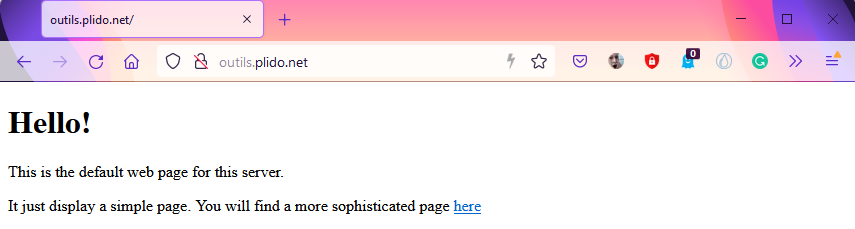
\includegraphics[width=1\columnwidth]{Pictures/firefox-simple.png}}
\lgf{\caption{Affichage de la page par Firefox}}
\lgf{\caption{Display of the page by Firefox}}
\label{fig-firefox-hello}
\end{figure}

  \vspace{1em}

% BE CAREFULL WITH WIRESHARK MENU TRANSLATION
\lgf{Wireshark a permis de visualiser le trafic échangé entre l'ordinateur et le serveur Web. Le trafic doit être similaire a celui de la figure~\vref{fig-wires-cap}. La figure s'obtient en sélectionnant le menu \textit{Statistiques/Graphique de flux} et en cochant \textit{Limiter au Filtre d'Affichage}. Elle est un peu plus lisible car elle représente les échanges sous forme de chronographes.}
\lge{Wireshark allowed to visualize the traffic exchanged between the computer and the Web server. The traffic should be similar to the one in the figure~\vref{fig-wires-cap}. The figure is obtained by selecting the menu \textit{Statistics/Flow Graph} and checking \textit{Limit to Display Filter}. It is a little more readable because it represents the exchanges in the form of time diagrams.}

\begin{figure}[tbp]
\centerline{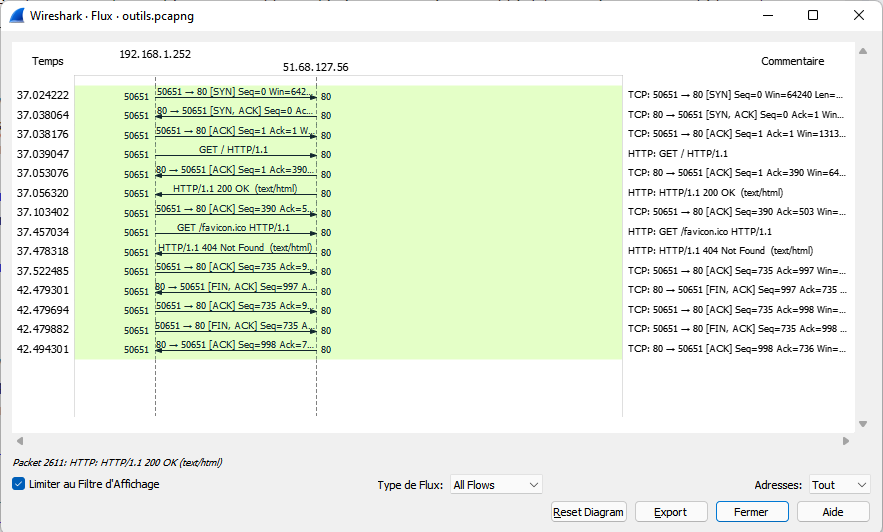
\includegraphics[width=1\columnwidth]{Pictures/ws-filtre.png}}
\lgf{\caption{Diagramme temporel des échanges.}}
\lge{\caption{Time diagram of exchanges.}}
\label{fig-ws-filtre}
\end{figure}

  \vspace{1em}

\lgf{Trois phases peuvent être distinguées~:}
\lge{Three phases can be distinguished:}

\begin{itemize}
    \item 
        \lgf{L'ouverture de connexion TCP avec l'émission de trois messages TCP~;}        
        \lge{TCP connection opening with the emission of three TCP~ messages;}
    \item 
        \lgf{la phase de transfert de données~:}
        \lge{the data transfer phase:}
    \begin{itemize}
        \item 
            \lgf{le client envoie une requête HTTP GET au serveur pour demander la ressource à la racine (\texttt{/}),}
            \lge{the client sends an HTTP GET request to the server to request the resource from the root (\texttt{/}),}
        \item 
            \lgf{le serveur acquitte le message au niveau TCP pour indiquer qu'il a bien été reçu.}
            \lge{the server acknowledges the message at the TCP level to indicate that it has been received.}
        \item 
            \lgf{le serveur envoie la réponse à la requête précédente et précisant le statut (\textttt{200 : OK}) et le que contenu est formaté en HTML.}
            \lge{the server sends the answer to the previous request and specifying the status (\textttt{200 : OK}) and the content is formatted in HTML.}
        \item 
            \lgf{le client acquitte ce message au niveau TCP,}
            \lge{the client acknowledges this message at the TCP level,}
        \item 
            \lgf{le client envoie une nouvelle requête HTTP GET pour obtenir la ressource \texttt{/facicon.ico}}
            \lge{the client sends a new HTTP GET request to obtain the resource \texttt{/facicon.ico}}
        \item 
            \lgf{le serveur répond que la ressource n'existe pas (\texttt{404 : Not Found}). Cette requête acquitte implicitement le message précédent.}
            \lge{the server answers that the resource does not exist (\texttt{404 : Not Found}). This request implicitly acknowledges the previous message.}
        \item 
            \lgf{le client acquitte la réponse du serveur au niveau TCP.}
            \lge{the client acknowledges the server's response at the TCP level.}
    \end{itemize}
    \item 
        \lgf{le serveur termine la connexion après 5 secondes d'inactivité. La fermeture se fait en échangeant 4 messages TCP.}
        \lge{the server ends the connection after 5 seconds of inactivity. The closing is done by exchanging 4 TCP messages.}
\end{itemize}

\Question{\lgf{Code de notification de HTTP}\lge{HTTP notification code}}
{
\lgf{Dans la trace suivante, nous avons vu que le serveur répondait aux requêtes du client par un numéro à 3 chiffres. A l'aide du \rfc{7231}, pouvez-vous attribuer le chiffre de gauche à une catégorie de notifications~:}
\lge{In the following trace, we saw that the server responded to client requests with a 3-digit number. Using the \rfc{7231}, can you assign the left digit to a category of notifications:}
  \vspace{1em}

\tabto{3cm}
\begin{description}
    \item    0 $\square$ \tab\tab $\square$ Redirection 
    \item    1 $\square$ \tab\tab $\square$ \lgf{Erreur coté serveur}\lge{Error on the server side}
    \item    2 $\square$ \tab\tab $\square$ \lgf{Erreur coté client}\lge{Error on the client side}
    \item    3 $\square$ \tab\tab $\square$ \lgf{Non attribué}\lge{Unassigned} 
    \item    4 $\square$ \tab\tab $\square$ \lgf{Succès}\lge{Success}
    \item    5 $\square$ \tab\tab $\square$ Information 
\end{description}

}
{
\begin{description}
    \item    0~: \lgf{Non attribué}\lge{Unassigned}
    \item    1~: Information 
    \item    2~: \lgf{Succès}\lge{Success}
    \item    3~: Redirection
    \item    4~: \lgf{Erreur coté client}\lge{Error on the client side}
    \item    5~: lgf{Erreur coté serveur}\lge{Error on the server side}
\end{description}}

\lgf{\subsection{Analyse des requêtes HTTP}}
\lge{\subsection{Analysis of HTTP requests}}

\lgf{La version 1.1 du protocole \ac{HTTP}  est spécifiée par le \rfc{7230}. Nous allons regarder une petite description en anglais de l'architecture et des formats des messages.}
\lge{The version 1.1 of the protocol \ac{HTTP} is specified by the \rfc{7230}. We will look at a small description in English of the architecture and the formats of the messages.}

\begin{termc} [basicstyle=\footnotesize\ttfamily, frame=single]

2.  Architecture

  HTTP was created for the World Wide Web (WWW) architecture and has
  evolved over time to support the scalability needs of a worldwide
  hypertext system.  Much of that architecture is reflected in the
  terminology and syntax productions used to define HTTP.

2.1.  Client/Server Messaging

  HTTP is a stateless request/response protocol that operates by
  exchanging messages  across a reliable transport- or
  session-layer "connection".  An HTTP "client" is a
  program that establishes a connection to a server for the purpose of
  sending one or more HTTP requests.  An HTTP "server" is a program
  that accepts connections in order to service HTTP requests by sending
  HTTP responses.

\end{termc}

\Question{\lgf{Organisme de standardisation.}\lge{Standardization body.}}
{
\lgf{Quelle organisation de standardisation a publié ce document ?}
\lge{Which standards organization published this document?}

\begin{itemize}[label=$\circ$]
   \item \Wrong{Microsoft}
   \item \Wrong{ISO}
   \item \Wrong{IEEE}
   \item \Correct{IETF}
 \end{itemize}
}
{
\lgf{Le préfixe \acl{RFC} est caractéristique de l'IETF.}
\lge{The prefix \acl{RFC} is characteristic of the IETF.}
}

\lgf{Le RFC indique ensuite~:}
\lgf{The RFC then states~:}

\begin{termc} [basicstyle=\footnotesize\ttfamily, frame=singlelabel={lst-rfc7230}]
  The terms "client" and "server" refer only to the roles that these
  programs perform for a particular connection.  The same program might
  act as a client on some connections and a server on others. [...]
 
  Most HTTP communication consists of a retrieval request (GET) for a
  representation of some resource identified by a URI.  In the simplest
  case, this might be accomplished via a single bidirectional
  connection (===) between the user agent (UA) and the origin
  server (O).

           request   >
      UA ======================================= O
                                  <   response

  A client sends an HTTP request to a server in the form of a request
  message, beginning with a request-line that includes a method, URI,
  and protocol version, followed by header fields
  containing request modifiers, client information, and representation
  metadata, an empty line to indicate the end of the
  header section, and finally a message body containing the payload
  body.

  A server responds to a client's request by sending one or more HTTP
  response messages, each beginning with a status line that includes
  the protocol version, a success or error code, and textual reason
  phrase possibly followed by header fields containing
  server information, resource metadata, and representation metadata,
  an empty line to indicate the end of the header
  section, and finally a message body containing the payload body.

  The following example illustrates a typical message exchange for a
  GET request on the URI "http://www.example.com/hello.txt":

  Client request:

    GET /hello.txt HTTP/1.1
    User-Agent: curl/7.16.3 libcurl/7.16.3 OpenSSL/0.9.7l zlib/1.2.3
    Host: www.example.com
    Accept-Language: en, mi

  Server response:

    HTTP/1.1 200 OK
    Date: Mon, 27 Jul 2009 12:28:53 GMT
    Server: Apache
    Last-Modified: Wed, 22 Jul 2009 19:15:56 GMT
    ETag: "34aa387-d-1568eb00"
    Accept-Ranges: bytes
    Content-Length: 51
    Vary: Accept-Encoding
    Content-Type: text/plain

    Hello World! My payload includes a trailing CRLF.
\end{termc}

\Question{\lgf{Formatage des messages HTTP}\lge{Formatting HTTP messages}}
{
\lgf{Est-ce que les en-têtes HTTP ont une taille fixe (vous pouvez aller voir le \rfc{7231} qui donne des indications sur le protocole) ?}
\lge{Do HTTP headers have a fixed size (you can check the \rfc{7231} which gives indications on the protocol)?}
\begin{itemize}[label=$\circ$]
   \item \Wrong{
    \lgf{l'en-tête tient en une ligne de 80 caractères.}
    \lge{the header is one line of 80 characters.}
    }
   \item \Correct{
    \lgf{une ligne blanche sépare l'en-tête du contenu. L'en-tête peut contenir autant de lignes que nécessaire. }
    \lge{a blank line separates the header from the content. The header can contain as many lines as necessary. }
    }
 \end{itemize}
}
{
\lgf{Comme on le voit sur l'exemple donné dans le RFC pour le message de réponse, l'en-tête HTTP contient, une ligne obligatoire, suivie d'options. Leur nombre n'est pas fixé par le standard. pour les séparer des données, une ligne blanche fait office de séparation.}
\lge{As we can see on the example given in the RFC for the response message, the HTTP header contains a mandatory line, followed by options. Their number is not fixed by the standard. To separate them from the data, a blank line acts as a separation.}
}

\Question{\lgf{Options des en-têtes HTTP}\lge{HTTP Header Options}}
{
\lgf{Comment sont construites les lignes optionnelles de l'en-tête ?}
\lge{How are the optional lines in the header constructed?}
\begin{itemize}[label=$\circ$]
   \item \Correct{
    \lgf{mot-clé : valeurs}
    \lge{keyword : values}
    }
   \item \Wrong{
    \lgf{un texte non formaté}
    \lge{unformatted text}
    }
   \item \Wrong{
    \lgf{mot-clé : longueur des données : valeurs}
    \lge{keyword : data length : values}
    }
 \end{itemize}
}
{
\lgf{L'en-tête est de taille variable. Elle comporte une première ligne obligatoire donnant la nature de la requête ou de la réponse, suivie d'informations optionnelles construites sur le format "mot clé : valeur". Une ligne blanche sépare l'en-tête du contenu.}
\lge{The header is of variable size. It has a mandatory first line giving the nature of the request or response, followed by optional information built on the "keyword: value" format. A blank line separates the header from the content.}
}

\lgf{\subsection{Analyse de la pile protocolaire}}
\lge{\subsection{Protocol stack analysis}}

\lgf{La trame contenant la requête HTTP GET permet de visualiser l'encapsulation protocolaire définie par le modèle de référence de l'\ac{ISO}. Dans Wireshark, en cliquant sur la trame, on peut la voir désassemblée et en hexadécimal dans les deux fenêtres comme le montre la figure~\vref{fig-ws-GET}.}
\lge{The frame containing the HTTP GET request allows to visualize the protocol encapsulation defined by the reference model of the ISO. In Wireshark, by clicking on the frame, we can see it disassembled and in hexadecimal in both windows as shown in the figure~\vref{fig-ws-GET}.}

\begin{figure}[tbp]
\centerline{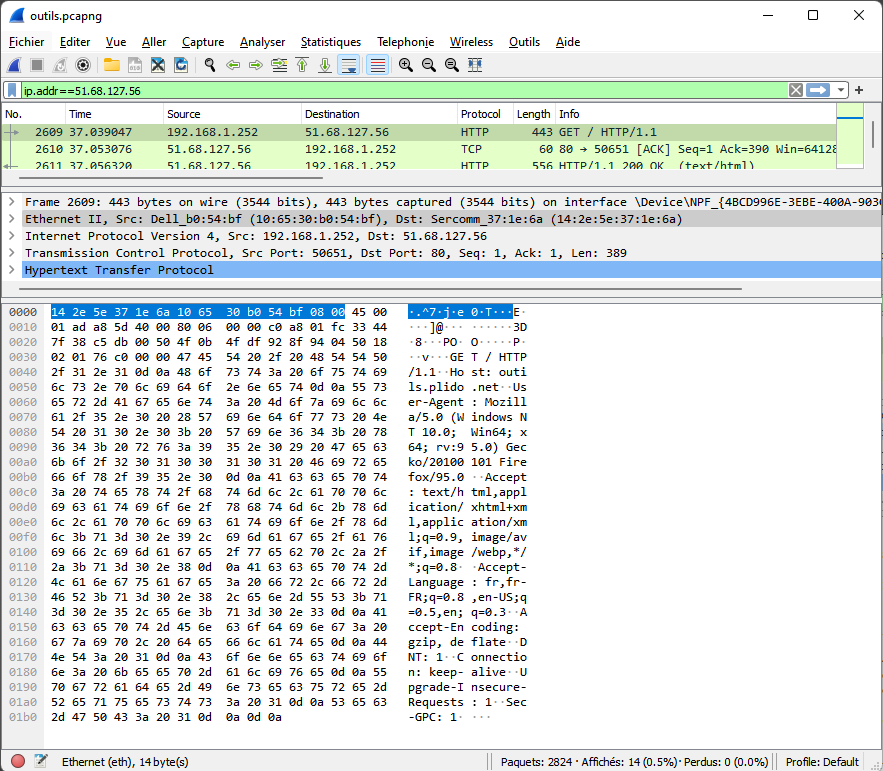
\includegraphics[width=1\columnwidth]{Pictures/ws-GET.png}}
\lgf{\caption{Contenu de la trame transportant la requête HTTP GET}}
\lge{\caption{Content of the frame carrying the HTTP GET request}}
\label{fig-ws-GET}
\end{figure}

  \vspace{1em}

\lgf{La deuxième fenêtre montre la pile protocolaire, inversée par rapport aux représentations classique (cf. figure~\vref{fig-fullstack}), mais correspondant à l'ordre des encapsulations dans la trame. Comment Wireshark a pu arriver à un tel résultat.}
\lge{The second window shows the protocol stack, inverted with respect to the classical representations (cf. figure~\vref{fig-fullstack}), but corresponding to the order of encapsulations in the frame. How Wireshark could arrive at such a result.}

\subsubsection{Ethernet}

\lgf{Wireshark reçoit une trame du réseau \Index{Ethernet} ou \Index{Wi-Fi}\footnote{Pour le réseau Wi-Fi, il transforme le format en celui d'une trame Ethernet pour un affichage plus compact.}. Le format d'un trame Ethernet est défini par le standard \Index{IEEE 802.3}. L'en-tête contient trois champs~:}
\lge{Wireshark receives a frame from the network \Index{Ethernet} or \Index{Wi-Fi}\footnote{For the Wi-Fi network, it transforms the format into that of an Ethernet frame for a more compact display}. The format of an Ethernet frame is defined by the standard \Index{IEEE 802.3}. The header contains three fields:}

\begin{itemize}
    \item 
        \lgf{6 octets pour l'adresse MAC du destinataire,}
        \lge{6 bytes for the MAC address of the destination,}
    \item 
        \lgf{6 octets pour l'adresse de la source,}
        \lge{6 bytes for the source address,}
    \item 
        \lgf{2 octets pour le protocole de niveau supérieur. Ainsi la valeur \texttt{0x0800} désigne IPv4 et \texttt{0x86dd} IPv6.}
        \lge{2 bytes for the higher level protocol. Thus the value \texttt{0x0800} indicates IPv4 and \texttt{0x86dd} IPv6.}
\end{itemize}

  \vspace{1em}

\lgf{Suivant le principe du modèle de référence de l'ISO, les adresses sont celles des nœuds adjacents, c'est-à-dire connecté au même réseau Ethernet ou Wi-Fi.}
\lge{Following the principle of the ISO reference model, the addresses are those of adjacent nodes, i.e. connected to the same Ethernet or Wi-Fi network.}

  \vspace{1em}

\lgf{Dans notre cas, le protocole de niveau supérieur est donc un paquet IPv4 et Wireshark peut continuer à analyser, ce qui suit. Formellement se sont des données de la trame Ethernet, mais elles peuvent être comprise comme un paquet IPv4.}
\lge{In our case, the top level protocol is therefore an IPv4 packet and Wireshark can continue to analyze this. Formally it is data from the Ethernet frame, but it can be understood as an IPv4 packet.}

\Question{\lgf{Mon adresse}\lge{My address}}
{
\lgf{Dans l'exemple, figure~\vref{fig-ws-GET}, qu'elle est l'adresse Ethernet de la machine émettrice de la trame ?}
\lge{In the example, figure~\vref{fig-ws-GET}, what is the Ethernet address of the machine sending the frame?}
}{
\lgf{\texttt{10:65:30:b0:54:bf}. Attention, la trame commence par l'adresse de la destination, suivie de l'adresse de la source.}
\lge{\texttt{10:65:30:b0:54:bf}. Be careful, the frame starts with the destination address, followed by the source address.}
}

\subsubsection{IPv4}

\lgf{Le format des paquets IPv4 défini dans le \rfc{791} a très peu évolué depuis sa publication en 1981. La figure~\vref{fig-header-IPv4} reprend ce format. Sans entrer dans les détails, les champs~:}
\lge{The IPv4 packet format defined in the \rfc{791} has changed very little since its publication in 1981. Figure~\vref{fig-header-IPv4} shows this format. Without going into detail, the fields~:}

\begin{itemize}
    \item 
        \lgf{adresse \texttt{source} et \texttt{destination} vont contenir les adresses IPv4 sur 32 bits des équipements d'extrémité. Des équipements intermédiaires, appelés routeur se chargent de recopier le paquet vers sa destination.}
        \lge{Addresses \texttt{source} and \texttt{destination} will contain the IPv4 addresses on 32 bits of the end equipment. Intermediary equipments, called routers are in charge of copying the packet to its destination.}
    \item 
        \lgf{Le champ \texttt{protocole} désigne la couche supérieure, la valeur 6 correspond à \Index{TCP} et 17 à \Index{UDP}.}
        \lge{The field \texttt{protocol} designates the upper layer, the value 6 corresponds to \Index{TCP} and 17 to \Index{UDP}.}
\end{itemize}

\begin{figure}[tbp]

	\center {
    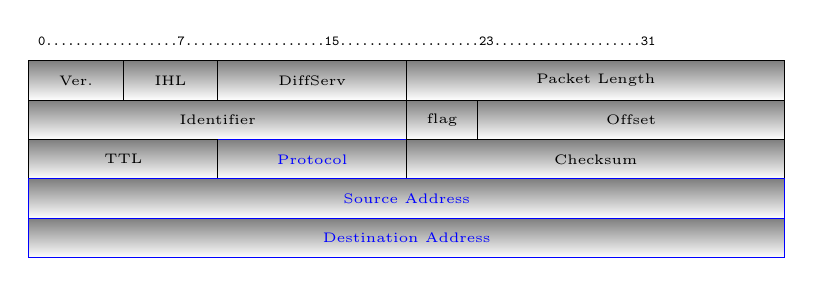
\begin{tikzpicture}

	\draw (0.5, 5.5) node  [right] {\tiny{\tt{0..................7...................15...................23....................31}}};
	
	 \draw (0.5, 5) node (context) [right, shade,  draw, minimum height=0.5cm, minimum width=1.2cm] {\tiny{Ver.}};

	\draw (1.7, 5) node (context) [right, draw, shade, minimum height=0.5cm, minimum width=1.2cm] {\tiny{IHL}};

	 \draw (2.9, 5) node (context) [right, draw, shade,  minimum height=0.5cm, minimum width=2.4cm] {\tiny{DiffServ}};

	 \draw (5.3, 5) node (context) [right, draw, shade,  minimum height=0.5cm, minimum width=4.8cm] {\tiny{Packet Length}};

	 \draw (0.5, 4.5) node (context) [right, draw, shade,  minimum height=0.5cm, minimum width=4.8cm] {\tiny{Identifier}};
	 \draw (5.3, 4.5) node (context) [right, draw, shade,  minimum height=0.5cm, minimum width=.9cm] {\tiny{flag}};
	 \draw (6.2, 4.5) node (context) [right, draw, shade,  minimum height=0.5cm, minimum width=3.9cm] {\tiny{Offset}};

	 \draw (2.9, 4) node (context) [right, draw, shade,  minimum height=0.5cm, minimum width=2.4cm, blue] {\tiny{Protocol}};

	 \draw (0.5, 4) node (context) [right, draw, shade,  minimum height=0.5cm, minimum width=2.4cm] {\tiny{TTL}};

	 \draw (5.3, 4) node (context) [right, draw, shade,  minimum height=0.5cm, minimum width=4.8cm] {\tiny{Checksum}};
	 
	 \draw (0.5, 3.5) node (context) [right, draw, shade,  minimum height=0.5cm, minimum width=9.6cm, blue] {\tiny{Source Address}};
	 \draw (0.5, 3) node (context) [right, draw, shade,  minimum height=0.5cm, minimum width=9.6cm, blue] {\tiny{Destination Address}};


	\end{tikzpicture}
	} %\center

\lgf{\caption{Format d'un en-tête IPv4}}
\lge{\caption{Format of an IPv4 header}}
\label{fig-header-IPv4}
\end{figure}

\Question{\lgf{saut par saut}\lge{hop by hop}}
{
\lgf{Est-ce que l'adressse Ethernet \texttt{14:2e:5e:37:1e:6a} que l'on retrouve dans le paquet~\vref{fig-ws-GET} correspond à l'adresse Ethernet du destinataire du paquet ? A quoi correspond elle?}
\lge{Does the Ethernet address \texttt{14:2e:5e:37:1e:6a} found in the packet~\vref{fig-ws-GET} correspond to the Ethernet address of the recipient of the packet? What does it correspond to?}
}{
\lgf{Non, l'adresse Ethernet n'est valable que sur ce réseau Ethernet. Pour atteindre le destinataire le paquet devra traverser plusieurs routeurs. Comme la trame a été capturée sur la machine émettrice, cette adresse est donc celle du premier routeur traversé.}
\lge{No, the Ethernet address is only valid on this Ethernet network. To reach the recipient, the packet must cross several routers. As the frame was captured on the sending machine, this address is therefore that of the first router crossed.}
}

\subsubsection{TCP}

\lgf{Wireshark, à partir du champ protocole valant 0x06, détermine que les données IP qui suivent l'en-tête sont un message TCP, il peut donc poursuivre le désassemblage de la trame. Le format de l'en-tête TCP est donné figure~\vref{fig-header-TCP}. Les numéros de port déterminent quelle application est utilisée. Si un client va prendre un numéro quelconque (50651 dans la trace figure~\vref{fig-ws-GET}), les serveurs vont utiliser des numéros connus de tous. Ainsi, les serveur Web se vont vus attribuer la valeur 80. Ils peuvent en choisir d'autres, comme on l'a vu lors de la constructions des \ac{URL}. }
\lge{Wireshark, from the protocol field 0x06, determines that the IP data following the header is a TCP message, so it can continue disassembling the frame. The format of the TCP header is given in figure~\vref{fig-header-TCP}. The port numbers determine which application is used. If a client is going to use any number (50651 in the figure~\vref{fig-ws-GET}), the servers will use numbers known by all. Thus, the Web servers will be assigned the value 80. They can choose others, as we saw when building the \ac{URL}. }



\begin{figure}[tbp]

	\center {
    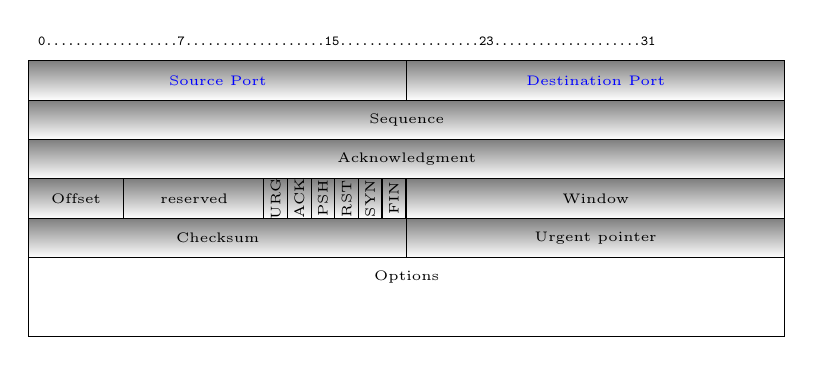
\begin{tikzpicture}

	\draw (0.5, 5.5) node  [right] {\tiny{\tt{0..................7...................15...................23....................31}}};
	
	 \draw (0.5, 5) node (SP) [right, shade,  draw, minimum height=0.5cm, minimum width=4.8cm] {};
	 \draw (SP) node [blue] {\tiny{Source Port}};

	 \draw (5.3, 5) node (DP) [right, shade,  draw, minimum height=0.5cm, minimum width=4.8cm] {};
	 \draw (DP) node [blue] {\tiny{Destination Port}};
	 
	 \draw (0.5, 4.5) node (seq) [right, shade,  draw, minimum height=0.5cm, minimum width=9.6cm] {};
	 \draw (seq) node  {\tiny{Sequence}};	 

	 \draw (0.5, 4) node (ack) [right, shade,  draw, minimum height=0.5cm, minimum width=9.6cm] {};
	 \draw (ack) node  {\tiny{Acknowledgment}};	 

	 \draw (0.5, 3.5) node (offset) [right, shade,  draw, minimum height=0.5cm, minimum width=1.2cm] {};
	 \draw (offset) node  {\tiny{Offset}};	 
	 
	 \draw (1.7, 3.5) node (res) [right, shade,  draw, minimum height=0.5cm, minimum width=1.8cm] {};
	 \draw (res) node  {\tiny{reserved}};	 
	 
	 \draw (5.3, 3.5) node (fin) [left, shade,  draw, minimum height=0.5cm, minimum width=0.3cm] {};
	 \draw (fin) node [rotate=90] {\tiny{FIN}};	 
	 \draw (5, 3.5) node (syn) [left, shade,  draw, minimum height=0.5cm, minimum width=0.3cm] {};
	 \draw (syn) node [rotate=90] {\tiny{SYN}};	 	 
	 \draw (4.7, 3.5) node (rst) [left, shade,  draw, minimum height=0.5cm, minimum width=0.3cm] {};
	 \draw (rst) node [rotate=90] {\tiny{RST}};	 	 
	 \draw (4.4, 3.5) node (psh) [left, shade,  draw, minimum height=0.5cm, minimum width=0.3cm] {};
	 \draw (psh) node [rotate=90] {\tiny{PSH}};	
	 \draw (4.1, 3.5) node (ack) [left, shade,  draw, minimum height=0.5cm, minimum width=0.3cm] {};
	 \draw (ack) node [rotate=90] {\tiny{ACK}};	
	 \draw (3.8, 3.5) node (urg) [left, shade,  draw, minimum height=0.5cm, minimum width=0.3cm] {};
	 \draw (urg) node [rotate=90] {\tiny{URG}};	
	 
	 \draw (5.3, 3.5) node (win) [right, shade,  draw, minimum height=0.5cm, minimum width=4.8cm] {};
	 \draw (win) node  {\tiny{Window}};	 	 
	 
	 \draw (0.5, 3) node (checksum) [right, shade,  draw, minimum height=0.5cm, minimum width=4.8cm] {};
	 \draw (checksum) node  {\tiny{Checksum}};

	 \draw (5.3, 3) node (urgent) [right, shade,  draw, minimum height=0.5cm, minimum width=4.8cm] {};
	 \draw (urgent) node  {\tiny{Urgent pointer}};

	 \draw (0.5, 2.5) node (option) [right,  draw, minimum height=1.5cm, minimum width=9.6cm] {};
	 \draw (option) node  {\tiny{Options}};	 	 
	 

	\end{tikzpicture}
	} %\center

\lgf{\caption{Format d'un en-tête TCP}}
\lge{\caption{Format of a TCP header}}
\label{fig-header-TCP}
\end{figure}


\lgf{Wireshark connaît cette liste de numéro de port bien connu et peut continuer à analyser la trame comme étant du HTTP.}
\lge{Wireshark knows this list of well-known port numbers and can continue to parse the frame as HTTP.}

\lgf{Sans entrer dans les détails, on peut aussi remarquer une série de valeurs binaires qui servent par exemple à ouvrir ou fermer une connexion TCP. Si l'on reprend la phase d'ouverture de la connexion (cf. figure~\vref{fig-ws-filtre}), l'ouverture de connexion se fait par~:}
\lge{Without going into details, we can also notice a series of binary values which are used for example to open or close a TCP connection. If we go back to the opening phase of the connection (cf. figure~\vref{fig-ws-filter}), the connection is opened by~:}

\begin{itemize}
    \item 
        \lgf{l'émission par le client d'un message TCP avec le bit SYN de positionné,}
        \lge{the transmission by the client of a TCP message with the SYN bit set,}
    \item 
        \lgf{l'émission par le client d'un message TCP avec le bit SYN de positionné,}
        \lge{the transmission by the client of a TCP message with the SYN bit set,}
    \item 
        \lgf{le client répond en renvoyant un message avec le bit ACK de positionné.}
        \lge{the client responds by returning a message with the ACK bit set.}
\end{itemize}

\lgf{Ces trois messages qui ne contiennent pas de données servent à synchroniser la valeur initiale du champ \texttt{sequence} à chaque bout de la connexion.}
\lge{These three messages, which do not contain any data, are used to synchronize the initial value of the \texttt{sequence} field at each end of the connection.}
  
\Question{Fermeture de connexion}{
A l'aide de la figure~\vref{fig-ws-GET} ou de vos captures Wireshark, quels sont les messages impliqués dans la fermeture du connexion?}
{La fermeture de déconnexion nécessite l'envoie de quatre message. L'une des extrémité, par forcement celle qui a ouvert la connexion, envoie un message avec le bit FIN positionné. Il est acquitté par l'autre entité qui a son tour envoie un message avec le bit FIN positionné qui sera acquitté pour définitivement fermer la connexion.
}   

\section{Do it yourself}\label{chap-flask}

Un serveur Web peut s'écrire en Python grâce au module \Index{Flask}. Le programme \texttt{simple\_server.py} permet de créer un serveur Web sur son ordinateur.

 \pythonlst{simple\_server.py}
 
 Ce script nécessite quelques explications :

\begin{itemize}
    \item Limport ligne 1 importe l'objet Flask à partir du module flask.
    \item A la ligne 2 une instance d'un objet Flask, c'est-à-dire un serveur web, est créée. Un nom lui est associé à des fins de débogage.
    \item A la ligne 4 contient la partie la plus délicate du script. \texttt{@} est un décorateur qui est utilisé en python pour ajouter des propriétés à une fonction. Ici, nous associons un chemin d'URI et une méthode REST à la fonction qui est ensuite définie. De cette façon, lorsque le serveur Flash recevra une requête GET sur ce chemin d'URI, il appellera la fonction \texttt{hello\_word}.
    \item La fonction texttt{hello\_word} retourne simplement un texte que le navigateur affichera.
    \item le serveur est lancé, ligne 8, en appelant la methode \pfunction{Flask}{run}. Il va attendre sur toutes les interfaces (adresse joker \texttt{0.0.0.0}) et sur le port 8080. 
\end{itemize}

  \vspace{1em}

Pour lancer le serveur, vous devez d'abord installer le module \texttt{Flask} avec \texttt{\Index{pip}}.

\begin{termc}[backgroundcolor=\color{palerod}, language=json, basicstyle=\ttfamily\small, escapechar=@]
# @\textbf{pip3 install Flask}@
Collecting Flask
  Downloading Flask-2.0.2-py3-none-any.whl (95 kB)
     |                                  | 95 kB 4.3 MB/s 
Collecting Jinja2>=3.0
  Downloading Jinja2-3.0.3-py3-none-any.whl (133 kB)
...
\end{termc}

  \vspace{1em}

Une fois le paquetage installé, il suffit d'exécuter le programme:
\begin{termc}[backgroundcolor=\color{palerod}, language=json, basicstyle=\ttfamily\small, escapechar=@]
# @\textbf{python3.9 simple\_server.py}@
 * Serving Flask app 'My First Web Server' (lazy loading)
 * Environment: production
   WARNING: This is a development server. Do not use it in a production
   deployment.
   Use a production WSGI server instead.
 * Debug mode: off
 * Running on all addresses.
   WARNING: This is a development server. Do not use it in a production
   deployment.
 * Running on http://192.168.1.53:8080/ (Press CTRL+C to quit)
127.0.0.1 - - [14/Dec/2021 21:06:55] "GET / HTTP/1.1" 200 -
127.0.0.1 - - [14/Dec/2021 21:06:59] "GET /favicon.ico HTTP/1.1" 404 -
\end{termc}


\Question{loopback}
{Quelle URI devez vous entrer dans votre navigateur pour accéder en local à ce serveur.}
{L'adresse de loopback est \texttt{127.0.0.1} et le port est 8080, le chemin d'URI est \texttt{/}. L'URI est donc \texttt{http://127.0.0.1:8080/}.}

\Question{Nom du serveur}{
A l'aide de Wireshark, pouvez vous déterminer dans la réponse les valeurs des options HTTP \texttt{\Index{Content-Type}} et \texttt{Server}.

Ne pas oublier que le trafic passe par l'interface \textit{loopback}. Pour afficher le trafic sur un port particulier, vous pouvez utiliser le filtre \texttt{tcp.port==XXXX}.
}{
On trouve les valeurs suivantes~:
\begin{itemize}
    \item \texttt{Server: Werkzeug/2.0.2 Python/3.9.6}
    \item \texttt{Content-Type: text/html; charset=utf-8}. La ressource est codée en HTML en utilisant un codage ASCII sur 8 bits.
\end{itemize}
}